\documentclass[MathsNotesBase.tex]{subfiles}

\date{\vspace{-6ex}}

\sloppy
\epstopdfsetup{outdir=./}
\graphicspath{ {./resources/img/LinearAlgebraOfPolynomials_images/} }

\begin{document}

\searchableSubsection{\sectionTitle{Linear Algebra of Polynomials}}{linear algebra, polynomials}{\bigskip}

\begin{par}
\begin{flushleft}
If we look for quadratic polynomials, $p\left(x\right)$, that pass throught the 3 points (1, 3), (3, 1) and (5, 2):
\end{flushleft}
\end{par}

\begin{center}
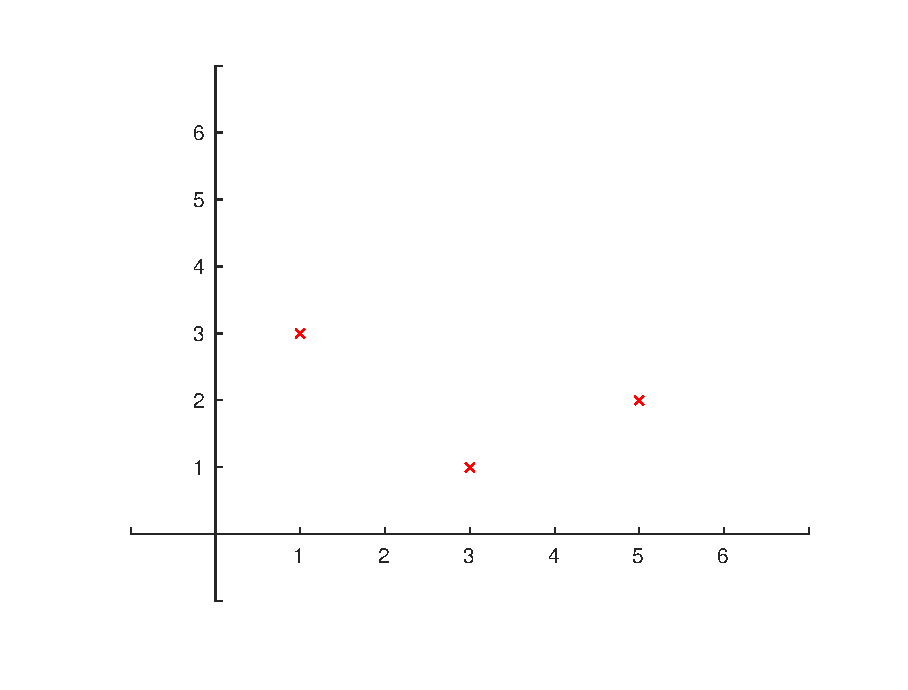
\includegraphics[width=\linewidth]{figure_0}
\end{center}


\begin{par}
\begin{flushleft}
Then the first has roots at $x=1,3$ and passes through the point (5, 2). So, we have:
\end{flushleft}
\end{par}

\begin{par}
$$p(1)=p(3)=0, p(5) = 2$$
\end{par}

\begin{par}
\begin{flushleft}
meaning that $\left(x-1\right)$and $\left(x-3\right)$are factors. Therefore,
\end{flushleft}
\end{par}

\begin{par}
$$\begin{array}{lcr}
&p(x) &= \alpha(x-1)(x-3)\\
&&= \alpha(x^2-4x+3)
\end{array}$$
\end{par}

\begin{par}
$$\begin{array}{lcr}
&p(5)&=2 \\
\Longrightarrow &\alpha(5^2-4(5) + 3) &= 2 \\
\iff &8\alpha&=2\\
\iff &\alpha &= \frac{1}{4}\\
\end{array}$$
\end{par}

\begin{par}
$$\therefore p(x) = \frac{1}{4}(x^2-4x+3)$$
\end{par}


\begin{center}
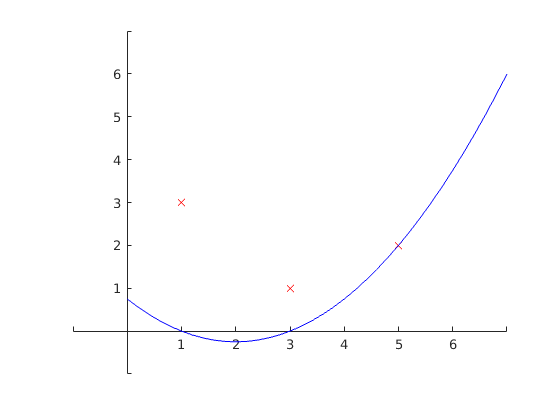
\includegraphics[width=\linewidth]{figure_1}
\end{center}


\begin{par}
\begin{flushleft}
The second has roots at $x=1,5$ and passes throught the point (3, 1):
\end{flushleft}
\end{par}

\begin{par}
$$\begin{array}{lcr}
&p(x) &= \alpha(x-1)(x-5)\\
&&= \alpha(x^2-6x+5)
\end{array}$$
\end{par}

\begin{par}
$$\begin{array}{lcr}
&p(3)&=1 \\
\Longrightarrow &\alpha(3^2-6(3) + 5) &= 1 \\
\iff &-4\alpha&=1\\
\iff &\alpha &= -\frac{1}{4}\\
\end{array}$$
\end{par}

\begin{par}
$$\therefore p(x) = -\frac{1}{4}(x^2-6x+5)$$
\end{par}


\begin{center}
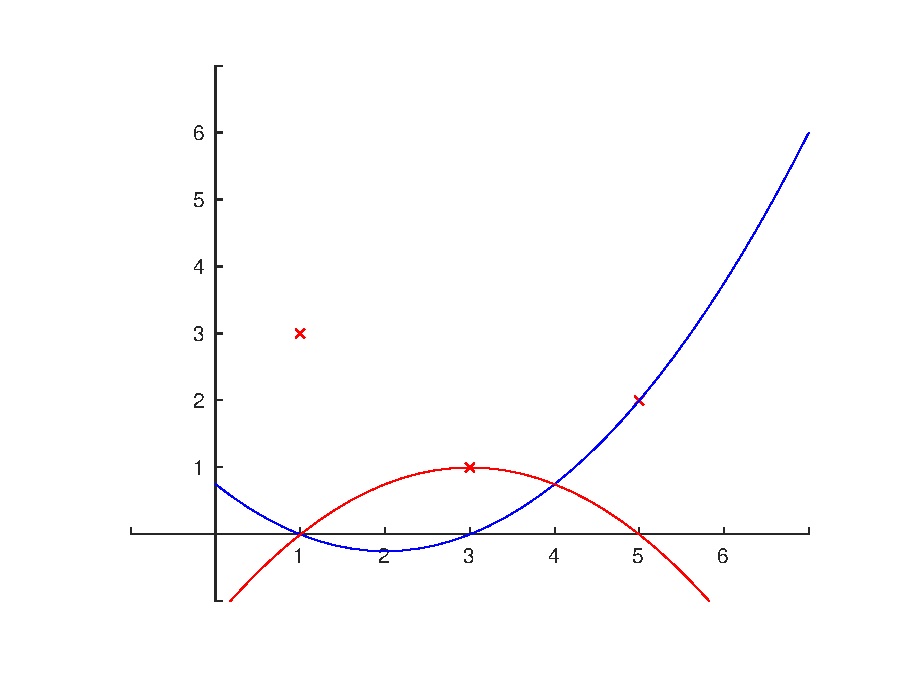
\includegraphics[width=\linewidth]{figure_2}
\end{center}


\begin{par}
\begin{flushleft}
The third has roots at $x=3,5$ and passes through the point (1, 3):
\end{flushleft}
\end{par}

\begin{par}
$$\begin{array}{lcr}
&p(x) &= \alpha(x-3)(x-5)\\
&&= \alpha(x^2-8x+15)
\end{array}$$
\end{par}

\begin{par}
$$\begin{array}{lcr}
&p(1)&=3 \\
\Longrightarrow &\alpha(1^2-8(1) + 15) &= 3 \\
\iff &8\alpha&=3\\
\iff &\alpha &= \frac{3}{8}\\
\end{array}$$
\end{par}

\begin{par}
$$\therefore p(x) = \frac{3}{8}(x^2-8x+15)$$
\end{par}


\begin{center}
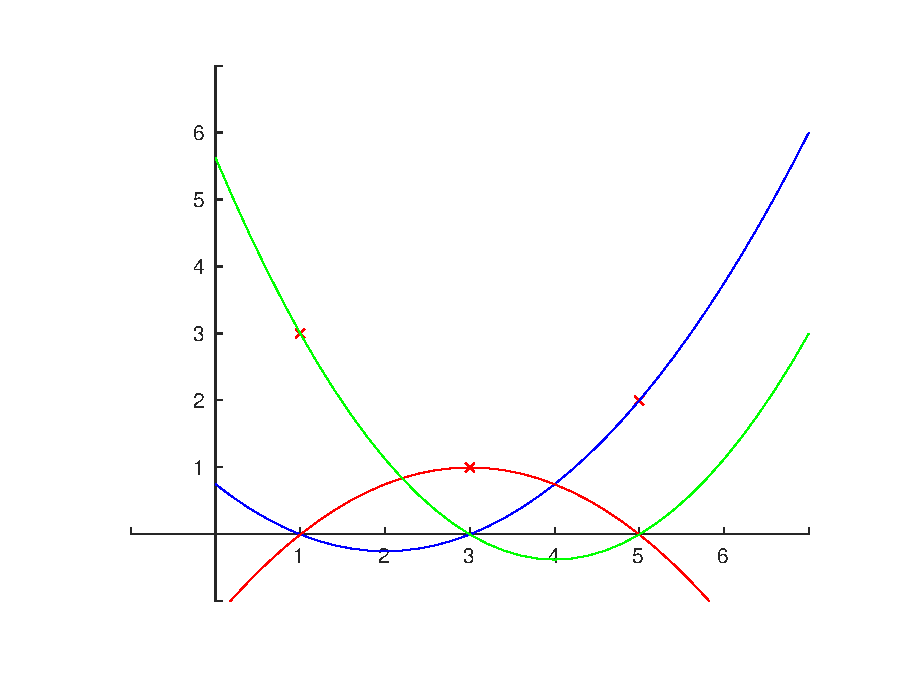
\includegraphics[width=\linewidth]{figure_3}
\end{center}


\begin{par}
\begin{flushleft}
Adding them together we get,
\end{flushleft}
\end{par}

\begin{par}
$$\begin{array}{lcr}
\;\;\;\;\; \frac{1}{4}(x^2-4x+3) - \frac{1}{4}(x^2-6x+5) + \frac{3}{8}(x^2-8x+15) \\[8pt]
= (\frac{1}{4}  - \frac{1}{4} + \frac{3}{8})x^2 + (-1 + \frac{6}{4} - 3)x + (\frac{3}{4} - \frac{5}{4} + \frac{45}{8}) \\[8pt]
= \;\; \frac{3}{8}x^2 - \frac{10}{4}x + \frac{41}{8} 
\end{array}$$
\end{par}


\begin{center}
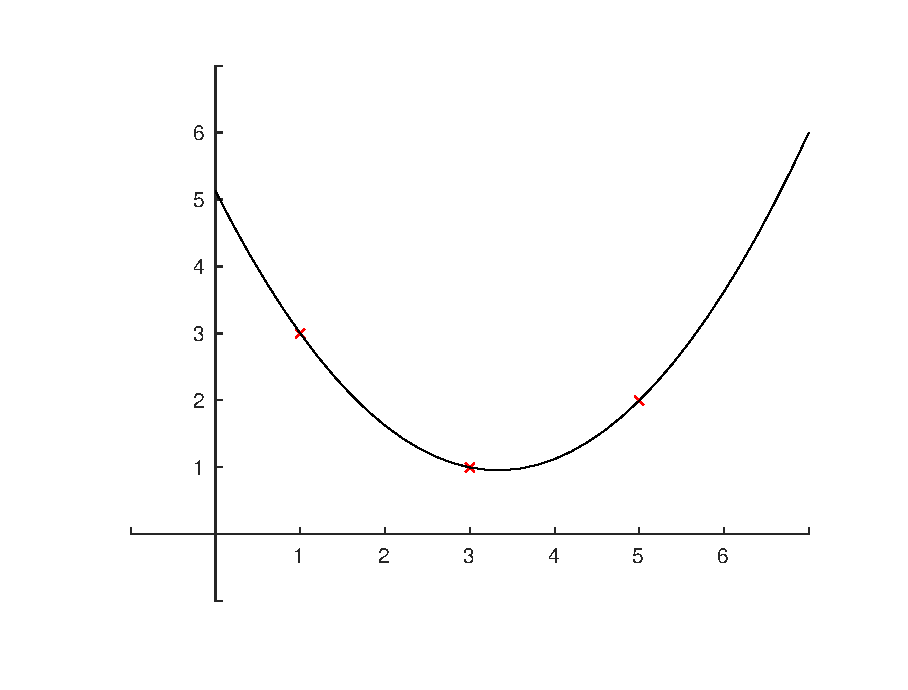
\includegraphics[width=\linewidth]{figure_4}
\end{center}

\end{document}
